%% genome_comparisons_expt.tex
%% Author: Leighton Pritchard
%% Copyright: James Hutton Institute
%% In vitro experimental whole genome comparisons

%
\begin{frame}
  \frametitle{Comparative Genomic Hybridisation}
  \begin{itemize}
    \item Two genomes: \textcolor{RawSienna}{reference} and \textcolor{hutton_green}{test} fragmented \& labelled
    \item Hybridise \textcolor{RawSienna}{reference} and \textcolor{hutton_green}{test} against a third \textcolor{hutton_blue}{"normal"} genome.
  \end{itemize}
  \begin{center}
    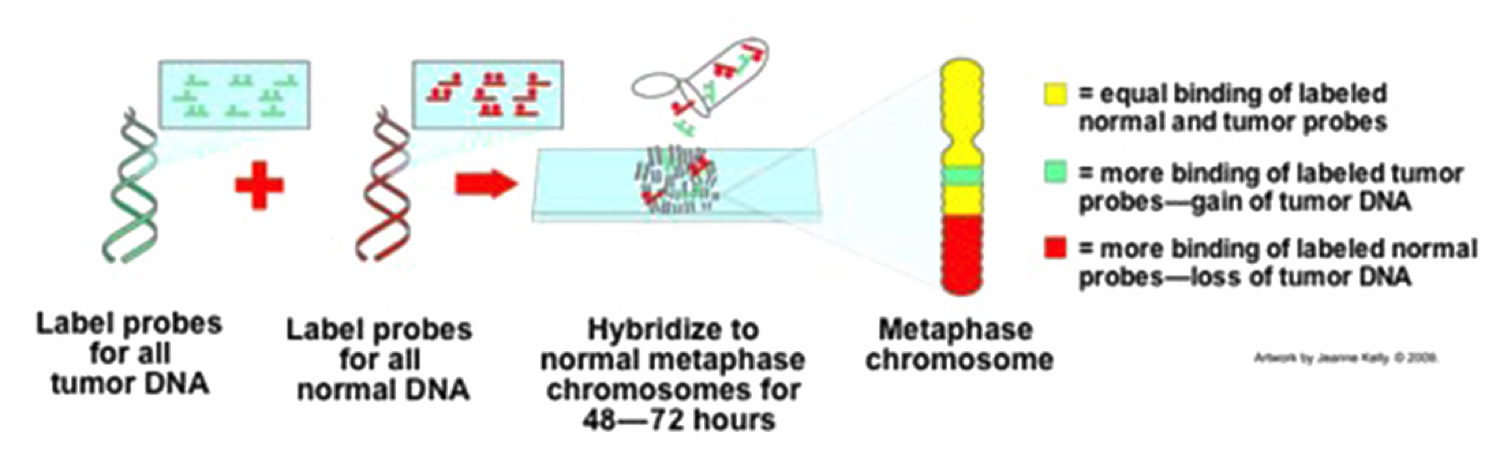
\includegraphics[width=\textwidth]{images/cgh}
  \end{center}  
  \begin{itemize}
    \item Differences in \textcolor{RawSienna}{red}/\textcolor{hutton_green}{green} intensity mapped by microscopy
    \item \textcolor{hutton_blue}{Colour intensity differences correspond to hybridisation, sequence similarity, and \textbf{copy number variations (CNV)}.}
    \item \textcolor{hutton_purple}{Can compare \textit{within} species/individuals (e.g. tumours), but labour-intensive, low-resolution}
  \end{itemize}  
\end{frame}

%
\begin{frame}
  \frametitle{CGH: epigenetics
  \footnote{\tiny{\href{http://dx.doi.org/10.1126/science.1359641
}{Kallionemi \textit{et al.} (1992) \textit{Science} doi:10.1099/10.1126/science.1359641
}}}
  \footnote{\tiny{\href{http://dx.doi.org/10.1073/pnas.0500398102
}{Fraga \textit{et al.} (2005) \textit{Proc. Natl. Acad. Sci. USA} doi:10.1073/pnas.0500398102
}}}
  }
  Measurements taken using image analysis - intensity on medial axis \\
  \textcolor{hutton_green}{Used for epigenetics: hybridisation of methylated DNA} \\
  \begin{columns}[T] 
    \column{.4\textwidth} 
      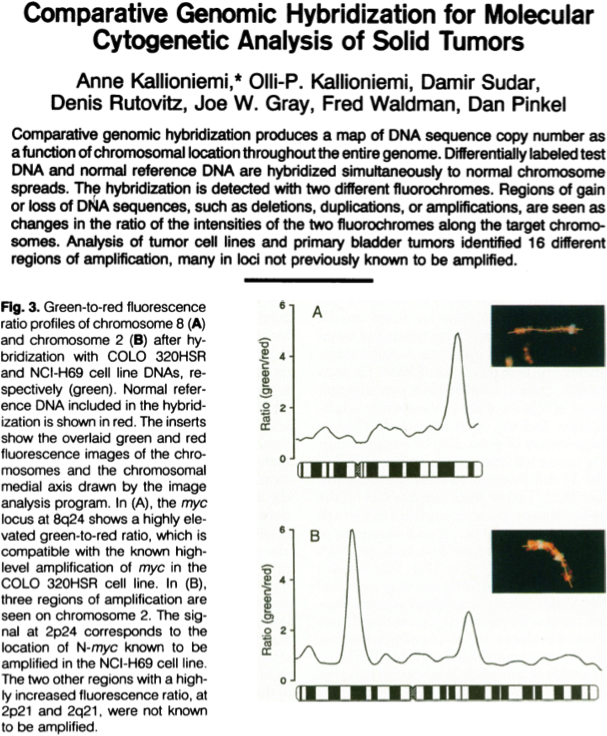
\includegraphics[width=\textwidth]{images/cgh_paper}
    \column{.4\textwidth}
      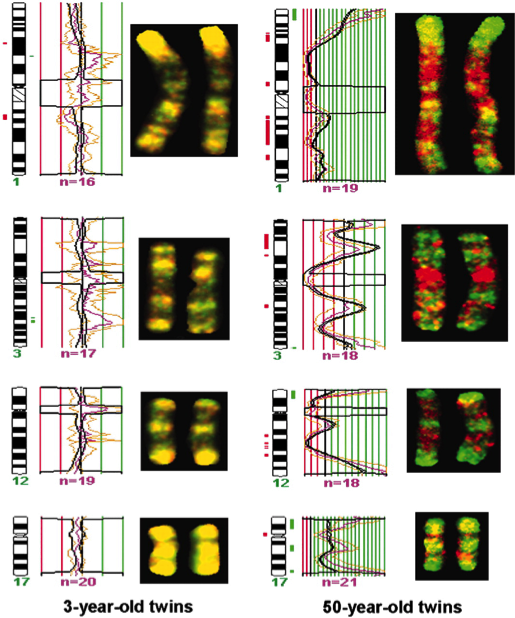
\includegraphics[width=\textwidth]{images/cgh_epigenetics}
  \end{columns}   
\end{frame}

%
\begin{frame}
  \frametitle{Array CGH (aCGH)
  \footnote{\tiny{\href{http://dx.doi.org/10.1038/12640
}{Pollack \textit{et al.} (1999) \textit{Nat. Genet.} doi:10.1099/10.1038/12640
}}}
  }
  Uses DNA microarrays: 1000s short, immobilised DNA probes \\
  gDNA, cDNA etc.\textcolor{RawSienna}{fluorescently}-\textcolor{hutton_green}{labelled} and hybridised to the array\\
  \begin{columns}[c] 
    \column{.4\textwidth} 
      \begin{itemize}
        \item Smaller sample sizes than CGH
        \item \textcolor{hutton_blue}{Automatable, high-throughput, high-resolution}
        \item \textcolor{hutton_purple}{Can identify copy number variation, segmental duplication, presence/absence}
      \end{itemize}
    \column{.6\textwidth}
      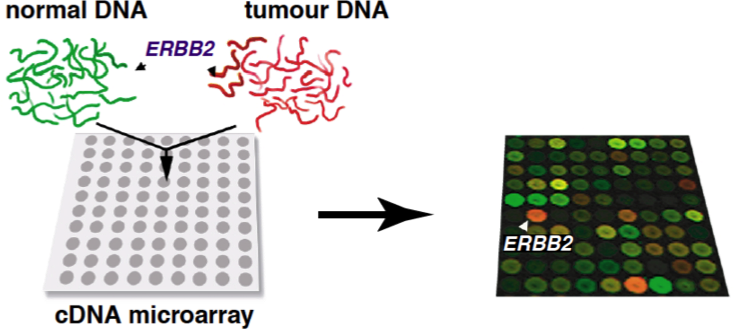
\includegraphics[width=\textwidth]{images/array_cgh}
  \end{columns}   
\end{frame}